% !TeX spellcheck = en_US
% !TeX encoding = ISO-8859-1

%#
%# ----------------------------------------------------------------------------
%#
%#  Copyright (C) 2014  Nuno AJ de Aniceto <nuno.aja@gmail.com>
%#
%#  This program is free software: you can redistribute it and/or modify
%#  it under the terms of the GNU General Public License as published by
%#  the Free Software Foundation, either version 3 of the License, or
%#  (at your option) any later version.
%#
%#  This program is distributed in the hope that it will be useful,
%#  but WITHOUT ANY WARRANTY; without even the implied warranty of
%#  MERCHANTABILITY or FITNESS FOR A PARTICULAR PURPOSE.  See the
%#  GNU General Public License for more details.
%#
%#  You should have received a copy of the GNU General Public License
%#  along with this program.  If not, see <http://www.gnu.org/licenses/>.
%#
%# ----------------------------------------------------------------------------
%#
%# If you have the interest, feel free to improve the script, contact me !
%#

% !TeX spellcheck = en_US
% !TeX encoding = ISO-8859-1

%#
%# ------------------------------------------------------------------------------
%#
%#    Copyright (C) 2014  Nuno AJ de Aniceto <nuno.aja@gmail.com>
%#
%#    This program is free software: you can redistribute it and/or modify
%#    it under the terms of the GNU General Public License as published by
%#    the Free Software Foundation, either version 3 of the License, or
%#    (at your option) any later version.
%#
%#    This program is distributed in the hope that it will be useful,
%#    but WITHOUT ANY WARRANTY; without even the implied warranty of
%#    MERCHANTABILITY or FITNESS FOR A PARTICULAR PURPOSE.  See the
%#    GNU General Public License for more details.
%#
%#    You should have received a copy of the GNU General Public License
%#    along with this program.  If not, see <http://www.gnu.org/licenses/>.
%#
%# ------------------------------------------------------------------------------
%#
%# If you have the interest, feel free to improve the script, contact me !
%#

% - - - - - - - - - - - - - - - - - - - - - - - - - - - - - - - - - - - - -
%
% 		package and document setups...
%
%

\documentclass[a4paper]{article}
%\documentclass[conference]{IEEEtran}

%\usepackage[cm]{fullpage}
\usepackage[margin=2.5cm]{geometry}
\usepackage{lipsum, blindtext}
\usepackage{texments, listings, minted}
\usepackage{fixltx2e, setspace, hyperref, framed, wrapfig, empheq}
\usepackage{graphicx, color, xcolor, fancyhdr, multicol}
\usepackage{braket, mathtools, amsmath, amsfonts, amssymb, mathtools}
\usepackage{array, booktabs, arydshln}
%\usepackage{arrayjob} % conflicts with array
\usepackage{tikz}
\usetikzlibrary{positioning, shapes}

% input & language internationalization
\usepackage[latin9]{inputenc}
%\usepackage[utf8]{inputenc}
\usepackage[T1]{fontenc}
\usepackage{eurosym}\def\texteuro{\euro}
\usepackage[english, portuguese]{babel}


% - - - - - - - - - - - - - - - - - - - - - - - - - - - - - - - - - - - - -
%
% 		setup based on template
%

\def \discipline 	{Decision Support Systems}
\def \articleId 	{3}

% author(s) & group
\def \groupId       {0}

\makeatletter
\author{
	Nuno Aniceto \\
	IST n. ????? \\
	\href{mailto:nuno.aja@gmail.com}{\texttt{nuno.aja@gmail.com}}
	\and
	Waldo \\
	IST n. ????? \\
	\href{mailto:???@??.com}{\texttt{???@??.com}}
}\let\Author\@author

% title & subtitle
\def \mainTitle 	{\discipline}
\def \subTitle 		{Homework \articleId{} - Group \groupId{}}

% pdf info
\pdfinfo{
	/Title    (\mainTitle - \subTitle)
	/Author   (Nuno AJ de Aniceto nuno.aja@gmail.com)
	/Subject  (Data Warehousing, Data Mining, Databases)
	/Keywords (Homework, SQL, Microsoft SQL Server)
}

% institute logotype location
\def \logotype 		{../@logos/ist_logo.png}

% !TeX spellcheck = en_US
% !TeX encoding = ISO-8859-1

%#
%# ------------------------------------------------------------------------------
%#
%#    Copyright (C) 2014  Nuno AJ de Aniceto <nuno.aja@gmail.com>
%#
%#    This program is free software: you can redistribute it and/or modify
%#    it under the terms of the GNU General Public License as published by
%#    the Free Software Foundation, either version 3 of the License, or
%#    (at your option) any later version.
%#
%#    This program is distributed in the hope that it will be useful,
%#    but WITHOUT ANY WARRANTY; without even the implied warranty of
%#    MERCHANTABILITY or FITNESS FOR A PARTICULAR PURPOSE.  See the
%#    GNU General Public License for more details.
%#
%#    You should have received a copy of the GNU General Public License
%#    along with this program.  If not, see <http://www.gnu.org/licenses/>.
%#
%# ------------------------------------------------------------------------------
%#
%# If you have the interest, feel free to improve the script, contact me !
%#

% - - - - - - - - - - - - - - - - - - - - - - - - - - - - - - - - - - - - -
%
% 		commands and environment setups...
%
%

% -- colors --
\definecolor{ist-blue}{HTML}{009DE0}
\definecolor{ist-gray}{HTML}{46555F}
\definecolor{answer-blue}{HTML}{009DE0}
\definecolor{answer-gray}{HTML}{46555F}


% -- matrix with different line-spacing --

\makeatletter
\renewcommand*\env@matrix[1][\arraystretch]{% \arraystretch
\edef\arraystretch{#1}%
	\hskip -\arraycolsep
	\let\@ifnextchar\new@ifnextchar
	\array{*\c@MaxMatrixCols c}}
\makeatother

% -- matrices and vectors --

%\begingroup
%\renewcommand*{\arraystretch}{1.5}
% (pmatrix expression here)
%\endgroup

% 2/3d column-vectors \cvec[a]{b}{c} or \cvec{x}{y}
\newcommand*\cvec[3][]{
    \begin{pmatrix}\ifx\relax#1\relax\else#1\\\fi#2\\#3\end{pmatrix}
}

% -- boxes --

\newenvironment{bb}{\empheq[box=\boxed]{flalign*}{\textbf{Answer}}\\[10pt]} {\endempheq{\\[10pt]}}


% -- inline boxing an important equation (counter) --

\newcommand*\textfbox[2][equation title]{%
  \begin{tabular}[b]{@{}c@{}}#1\\\fbox{#2}\end{tabular}}

% -- usage example --
% \begin{empheq}[box={\textfbox[A different equation title]}]{align}
%   important equation #x (with counter)
% \end{empheq}


% -- avoid indentation (on itemizations, enumerations, listings, etc) --
% problem: does not allow spanning over several pages - to be resolved !
\newcommand\NoIndent[1]{
  \par\vbox{\parbox[t]{\linewidth}{#1}}
}

% -- answering to question with boxes --

%\makeatletter
%\newcommand{\answer}[1][(...answer here...) \\ \vspace{25pt}]{
%	\NoIndent{
%		\begin{center}
%				%%\begin{minipage}[c][4em][s]{\textwidth}
%				\begin{minipage}
%				{\dimexpr\linewidth-5\fboxsep-1\fboxrule\relax}
%					\centering{\textbf{\color{answer-blue}{Answer}}}\\[5pt]
%					\flushleft{\color{answer-gray}{#1}}
%				\end{minipage}
%		\end{center}
%	}
%	\vspace{25pt}
%}

%\makeatletter
\newcommand\answer[1][\par (...answer here...) \vs]{
	\noindent
	{
		\par
		\begin{center}
%			\centering{\textbf{\color{answer-blue}{Resposta}}}\\
			\flushleft{\color{answer-gray}{#1}}
		\end{center}
%		\flushleft
%		\par
	}
}
\newcommand\answerBox[1][(...answer here...) \\ \vspace{25pt}]{
	\noindent
	{
		\par
		\begin{center}
			\flushleft{\color{answer-gray}{#1}}
		\end{center}
		\par
	}
}

\makeatletter
\newcommand{\answerNI}[1][(...answer here...) \\ \vspace{25pt}]{
%	\begin{framed}
	\noindent
	{
		\begin{center}
			\centering{\textbf{\color{answer-blue}{Answer}}}\\
			\flushleft{\color{answer-gray}{#1}}
		\end{center}
	}
	\vspace{15pt}
%	\end{framed}
}

\makeatletter
\newcommand{\solution}[1][(...solution here...) \\ \vspace{25pt}]{
	%\begin{framed}
	\NoIndent
	{
		\begin{center}
			\centering{\textbf{\color{answer-blue}{Solution}}}\\
			\flushleft{\color{answer-gray}{{#1}}}
		\end{center}
	}
	\vspace{15pt}
	%\end{framed}
}


\newcommand\homework[1]{
	\begin{document}
	\maketitle \thispagestyle{empty}
	{#1}
	\end{document}
}

% % % % % % % % % % % % % % % % % % % % % % % % % % % % % % % % % % % % % %
%
% 	to test font types and set other options
%
%
%\makeatletter
%\newcommand*{\alphabet}{abcdefghijklmnopqrstuvwxyz}
%\newcommand*{\showalphabetwidth}[2]{%
%  \fontfamily{#1}\selectfont
%  \settowidth{\@tempdima}{\alphabet}%
%  \alphabet~-- width for #2 at 1\@ptsize pt: \the\@tempdima
%}
%\makeatother
%
%\showalphabetwidth{cmr}{Computer Modern}
%\showalphabetwidth{ptm}{Times New Roman}
%\showalphabetwidth{ppl}{Palatino}


%minipage:
%\hangindent=-2in
%\hangafter=5
%\usepackage{parskip}
%\setlength{\parindent}{5pt}
%
% % % % % % % % % % % % % % % % % % % % % % % % % % % % % % % % % % % % % %

% - - - - - - - - - - - - - - - - - - - - - - - - - - - - - - - - - - - - -
%
% 		document info and style setup:
%	 		title, author, date, headers, etc...
%
%


%\makeatletter
%\title{
%	\begin{center}
%		%
\includegraphics[scale=0.25]{ist_logo.png}\\
%		
\includegraphics[scale=0.4]{../@logos/ist_logo.png}\\
%		\vspace{20pt}
%		\hrulefill\\
%		\vspace{15pt}
%		\vspace{-100pt}
%		\textbf{Information and Computation for AI}\\
%		Homework \#7\\
%	\end{center}
%		\vspace{15pt}

\renewcommand*{\familydefault}{\sfdefault}

\makeatletter
\title{
		\vspace{-2cm}
		\begin{multicols}{2}
			\flushright
			\color{ist-gray}
			\textbf{\huge{\discipline}}\\{\Large \subTitle}\\
		\columnbreak
			\flushleft
			\includegraphics[scale=0.35]{\logotype}
		\end{multicols}
		\vspace{-1cm}
} \let\Title\@title

\date{
	\today \\
	\hrulefill\\
	\vspace{15pt}
} \let\Date\@date

%\fontfamily{ppl}\selectfont
%\renewcommand*{\familydefault}{\rmdefault}
%\renewcommand*{\familydefault}{\sfdefault}

\everymath{\displaystyle} 
\pagestyle{fancy}
\hypersetup{colorlinks=true, urlcolor=blue, unicode=true, linkcolor=blue}

\fancyhf{} % sets both header and footer to nothing
%\renewcommand{\headrulewidth}{0pt}


%\lhead{\authorName{} - \authorId}
\lhead{Grupo \groupId}
\chead{\includegraphics[scale=0.075]{\logotype}}
\rhead{p�gina $\thepage$}

\pagenumbering{arabic}

\newcommand{\vs}{\vspace{12pt}}
\newcommand{\hs}{\hspace{12pt}}
\parskip 		= 12pt
\baselineskip 	= 12pt

% define SQL script
%\begin{minted}[mathescape, linenos, numbersep=5pt, tabsize=4, xleftmargin=10pt,
%               xrightmargin=10pt, gobble=1, frame=single, framesep=2mm]{sql}
%	use AdventureWorksDW2012
%	
%	SELECT
%		SUM(SalesAmount)
%	FROM
%		FactInternetSales
%\end{minted}


%
%
% - - - - - - - - - - - - - - - - - - - - - - - - - - - - - - - - - - - - -

% - - - - - - - - - - - - - - - - - - - - - - - - - - - - - - - - - - - -

\begin{document}
%\selectlanguage{portuguese}
\selectlanguage{english}

\maketitle \thispagestyle{empty}
\flushleft

\begin{description}
\item[1)]{ \textbf{ (7pts) Defining Calculations}\par}
Link to the '\textit{Lesson 6: Defining Calculations}':\\
\url{http://technet.microsoft.com/en-us/library/db55e226-601a-4026-8651-573195555a59}
\par
After performing the '\textit{Lesson 6}' define calculations using \texttt{AdventureWorksDW2012} to perform the following query:\\
\vs
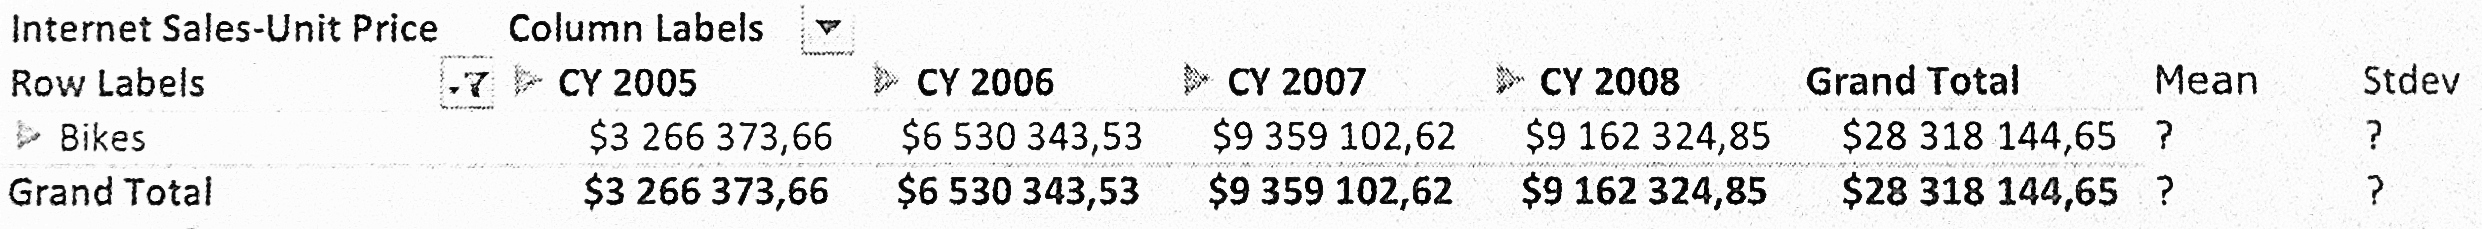
\includegraphics[scale=0.15]{img/question-1.png}

\begin{itemize}
\item[a) (1.5pts)] To compute the \textbf{mean value} of '\texttt{Bike Unit Price}' over four years as shown in the table, define calculations using the \texttt{CALCULATE} for \texttt{Internet Sales - Unit Price Amount}.\\
Indicate your script.\\
\answer
%\includegraphics[scale=0.75]{img/answer-1a}

\vs \item[b) (2.5pts)] To compute the \textbf{standard deviation} of the sample value of '\texttt{Bike Unit Price}' over four years as shown in the table, define calculations using the \texttt{CALCULATE} for \texttt{Internet Sales - Unit Price Amount}.\\
Indicate your script.\\

\answer
%\includegraphics[scale=0.75]{img/answer-1b}

\vs\item[c) (1pt)] Expand \texttt{Bikes} to \texttt{Mountain Bikes}, \texttt{Road Bikes}, \texttt{Touring Bikes} in the excel table with the \texttt{Grand Total}, \texttt{Mean Value}, \texttt{Standard deviation}.\\
Indicate the excel Table.\\

\answer

\vs
\end{itemize}

\newpage
\item[2)]{ \textbf{ (1pt) Normalization}\par}
Use \textbf{min-max} normalization to transfer the value $11$ of age into the range $[12 49]$.
\answer[{
The normalization will map then values from the range $A: [A_{min}, A_{max}]$ to the range $B: [B_{min}, B_{max}]$.\\
We assume that $A_{min}$ is of $0$ years - the aging of a person starts at the value of $0$.\\
And that $A_{max}$ is $11$ - considering the given value as the maximum value for the starting range.\\
The values of the counter domain $B$ are based on the given range.\\
Therefore we assume that the domain ($A$) and counter-domain ($B$) of this normalization are defined with the ranges: $A: [0, 11] \hs B: [12, 49]$.\\
\vs
The min-max normalization calculation is defined by the formula:\\
\vspace{2pt}
$b = \frac{B_{max} - B_{min}}{A_{max}-A_{min}}
		\cdot {(a - A_{min})} + B_{min}$ \\
\vs
Then we have:\\
\vs
$b = \frac{49 - 12}{11 - 0} \cdot {(11 - 0)} + 12 = 49$.\\
\vs
This value is expected to be $49$ (the maximum of $B$) as the min-max makes a linear interpolation between values from $A$ to values from $B$.\\
Because $11$ was considered the highest value $A$ could take, then it's mapping must be the highest value that $B$ could take: $49$.
}]

\vs
\item[3)]{ \textbf{ (5pts) PCA}\par}
Suppose we have the following points:\\
\vs
$\vec{x}_i =  \left\lbrace \cvec{0}{0}, \cvec{9}{1}, \cvec{1}{2},
\cvec{15}{1}, \cvec{11}{2}, \cvec{15}{3} \right\rbrace $\\
\begin{itemize}
\item[a) (2pts)] Compute the covariance matrix.
\answer

\vs
\item[b) (2pts)] What is the matrix of the K-L transformation ?
\answer
\vs
\item[c) (1pt)] Which of the two eigenvectors is more significant? Can we reduce the dimension?
\answer
\vs
\end{itemize}

\end{description}
\end{document}
